\documentclass[xcolor=table,aspectratio=169]{beamer}
\usetheme{Madrid}
\usepackage{adjustbox}
%\usetheme{metropolis}
\usepackage[style=verbose-note, sorting=none, sortcites=true, maxnames=1, giveninits=true, autocite=superscript, doi=false, url=false, isbn=false, backend=biber, citetracker=false, pagetracker=false, bibencoding=utf8, eprint=false]{biblatex}
% \usepackage[backend=bibtex,style=authoryear-comp,citestyle=authoryear-comp,firstinits=true,sorting=none,maxnames=1,doi=false,isbn=false,url=false,eprint=false]{biblatex}
\usepackage[T1]{fontenc}

\definecolor{twitter_blue}{HTML}{1da1f2}
% Definitions of colours used in seaborn for use in latex
\definecolor{seaborn_bg_grey}{HTML}{eaeaf2}
\definecolor{seaborn_bg_grey_dark}{HTML}{d2d2d9}
\definecolor{seaborn_bg_grey_darker}{HTML}{a3a3a9}
\definecolor{seaborn_bg_grey_half}{HTML}{f4f4f8}

\definecolor{seaborn_blue}{HTML}{4c72b0}
\definecolor{seaborn_green}{HTML}{55a868}
\definecolor{seaborn_red}{HTML}{c44e52}
\definecolor{seaborn_magenta}{HTML}{8172b2}
\definecolor{seaborn_yellow}{HTML}{ccb974}
\definecolor{seaborn_cyan}{HTML}{64b5cd}

\definecolor{seaborn_muted_blue}{HTML}{4878cf}
\definecolor{seaborn_muted_green}{HTML}{6acc65}
\definecolor{seaborn_muted_red}{HTML}{d65f5f}
\definecolor{seaborn_muted_magenta}{HTML}{b47cc7}
\definecolor{seaborn_muted_yellow}{HTML}{c4ad66}
\definecolor{seaborn_muted_cyan}{HTML}{77bedb}

\definecolor{seaborn_pastel_blue}{HTML}{92c6ff}
\definecolor{seaborn_pastel_green}{HTML}{97f0aa}
\definecolor{seaborn_pastel_red}{HTML}{ff9f9a}
\definecolor{seaborn_pastel_magenta}{HTML}{d0bbff}
\definecolor{seaborn_pastel_yellow}{HTML}{fffea3}
\definecolor{seaborn_pastel_cyan}{HTML}{b0e0e6}

\definecolor{seaborn_bright_blue}{HTML}{003fff}
\definecolor{seaborn_bright_green}{HTML}{03ed3a}
\definecolor{seaborn_bright_red}{HTML}{e8000b}
\definecolor{seaborn_bright_magenta}{HTML}{8a2be2}
\definecolor{seaborn_bright_yellow}{HTML}{ffc400}
\definecolor{seaborn_bright_cyan}{HTML}{00d7ff}

\definecolor{seaborn_dark_blue}{HTML}{001c7f}
\definecolor{seaborn_dark_green}{HTML}{017517}
\definecolor{seaborn_dark_red}{HTML}{8c0900}
\definecolor{seaborn_dark_magenta}{HTML}{7600a1}
\definecolor{seaborn_dark_yellow}{HTML}{b8860b}
\definecolor{seaborn_dark_cyan}{HTML}{006374}

\definecolor{seaborn_colorblind_blue}{HTML}{0072b2}
\definecolor{seaborn_colorblind_green}{HTML}{009e73}
\definecolor{seaborn_colorblind_red}{HTML}{d55e00}
\definecolor{seaborn_colorblind_magenta}{HTML}{cc79a7}
\definecolor{seaborn_colorblind_yellow}{HTML}{f0e442}
\definecolor{seaborn_colorblind_cyan}{HTML}{56b4e9}



% Gobbling first names

\AtEveryCitekey{%
   \clearfield{shorttitle}%
   \clearfield{month}%
   \ifentrytype{article}{%
      \clearfield{title}%
   }{}
   }
\ExecuteBibliographyOptions[online]{eprint=true}

% "blindfootcite" is the equivalent of "footcite" except the number marker does not appear
\newcommand\blfootcite[1]{%
  \begingroup
  \renewcommand\thefootnote{}\footnote{\hspace{-4ex}\cite{#1}}%
  \addtocounter{footnote}{-1}%
  \endgroup
}
\renewcommand*{\multicitedelim}{\textcolor{seaborn_bg_grey_darker}{\addsemicolon}}
\setbeamerfont{footnote}{size=\scriptsize}
\renewcommand\footnoterule{\kern-3pt \color{seaborn_bg_grey_darker}\hrule width \textwidth height 0.4pt \color{black} \kern 2.6pt}

\DeclareSourcemap{
  \maps[datatype=bibtex,overwrite=False]{
   \map{
     \step[fieldsource=journal,
           match={Journal of Chemical Theory and Computation},
           replace={JCTC}]
     \step[fieldsource=journal,
           match={Reviews of Modern Physics},
           replace={Rev. Mod. Phys.}]
     \step[fieldsource=journal,
           match={Reports on Progress in Physics},
           replace={Rep. Prog. Phys.}]
     \step[fieldsource=journal,
           match={Physical Review Letters},
           replace={Phys. Rev. Lett.}]
     \step[fieldsource=journal,
           match={Physical Review},
           replace={Phys. Rev.}]
     \step[fieldsource=journal,
           match={B - Condensed Matter and Materials Physics},
           replace={B}]
     \step[fieldsource=journal,
           match={Journal of Chemical Physics},
           replace={J. Chem. Phys.}]
     \step[fieldsource=journal,
           match={Annual Review of Materials Research},
           replace={Annu. Rev. Mater. Res.}]
   }
  }
}

\renewbibmacro{in:}{}
\DeclareFieldFormat{pages}{\mkfirstpage{#1}}
\beamertemplatenavigationsymbolsempty
\bibliography{zotero_library.bib}
\setbeamertemplate{bibliography item}[text]
\renewbibmacro{in:}{}
\AtEveryBibitem{\clearfield{title}}
\AtEveryBibitem{\clearfield{month}}
\AtEveryBibitem{\clearfield{pages}}
\DeclareNameAlias{default}{given-family}

% \renewcommand*{\bibfont}{\tiny}
\usepackage{amssymb}
\usepackage{epsfig}
\usepackage{psfrag}
\usepackage{wrapfig}
\usepackage{graphicx}
\usepackage{color}
\usepackage[table]{xcolor}
\usepackage{amsmath}
\usepackage{multimedia}
\usepackage{subcaption}
%\usepackage{style}
\usepackage{verbatim}
\usepackage{multicol}
\usepackage[table]{xcolor}
\usepackage{tabularx}
% Tikz
\usepackage{tikz}
\usetikzlibrary{positioning,shapes,arrows,backgrounds,fit,calc,external,trees,tikzmark}
% \tikzexternalize[prefix=tikzfigures/]
\tikzstyle{dummy} = []
\tikzstyle{line} = [draw, thick, -latex']
\tikzstyle{headless_line} = [draw, thick, -]
\tikzstyle{default}    = [rectangle, text centered, rounded corners, text=black, font=\sffamily\footnotesize, align=center]
\tikzstyle{default_text}    = [rectangle, text width=10cm, text=black,anchor=north west, font=\sffamily]
\tikzstyle{boxwhite} = [default, fill=white, rounded corners=0.1cm]
\tikzstyle{cp}    = [default, fill=seaborn_blue, text=white, text width=2.8cm, minimum height=0.5cm]
\tikzstyle{pw}    = [cp, fill=seaborn_green]
\tikzstyle{wannier90}    = [cp, fill=seaborn_cyan]
\tikzstyle{bespoke}    = [cp, fill=seaborn_magenta]
\tikzstyle{observable}    = [cp, fill=seaborn_red]
\tikzset{
  -|-/.style={
    to path={
      (\tikztostart) -| ($(\tikztostart)!#1!(\tikztotarget)$) |- (\tikztotarget)
      \tikztonodes
    }
  },
  -|-/.default=0.5,
  |-|/.style={
    to path={
      (\tikztostart) |- ($(\tikztostart)!#1!(\tikztotarget)$) -| (\tikztotarget)
      \tikztonodes
    }
  },
  |-|/.default=0.5,
}

\newlength{\myyshift}
\setlength{\myyshift}{0.05cm}

\usepackage{lipsum}
\usetikzlibrary{calc}
\newlength{\myfigscale}
\setlength{\myfigscale}{0.3cm}
\usepackage{smartdiagram}
\usesmartdiagramlibrary{additions}
\usepackage{multicol}
\usepackage{helvet}
% \usepackage{sansmath}
% \sansmath
\usepackage{cancel} % for \cancel
\usepackage[normalem]{ulem} % for sout (strike out)
\usepackage{tcolorbox}
\tcbuselibrary{skins,hooks}
\tcbset{colframe=structure,fonttitle=\bfseries,beamer, clip upper, boxsep=0pt, sharp corners=all, no shadow, left skip=0pt, right skip=0pt, coltext=white}

% For electron orbital diagrams
\usepackage{tikzorbital}
% Changing defaults
\pgfkeys{tikzorbital/drawLevel/width = 0.666666}
\pgfkeys{tikzorbital/drawLevel/style = {line width = 1pt, color = black!80, line cap = round}}
\pgfkeys{tikzorbital/drawLevel/spinlength = 0.666666}
\pgfkeys{tikzorbital/drawLevel/spinstyle = {very thick, color = black!80, -stealth}}

% Definitions of colours used in seaborn for use in latex
\definecolor{seaborn_bg_grey}{HTML}{eaeaf2}
\definecolor{seaborn_bg_grey_dark}{HTML}{d2d2d9}
\definecolor{seaborn_bg_grey_darker}{HTML}{a3a3a9}
\definecolor{seaborn_bg_grey_half}{HTML}{f4f4f8}

\definecolor{seaborn_blue}{HTML}{4c72b0}
\definecolor{seaborn_green}{HTML}{55a868}
\definecolor{seaborn_red}{HTML}{c44e52}
\definecolor{seaborn_magenta}{HTML}{8172b2}
\definecolor{seaborn_yellow}{HTML}{ccb974}
\definecolor{seaborn_cyan}{HTML}{64b5cd}

\definecolor{seaborn_muted_blue}{HTML}{4878cf}
\definecolor{seaborn_muted_green}{HTML}{6acc65}
\definecolor{seaborn_muted_red}{HTML}{d65f5f}
\definecolor{seaborn_muted_magenta}{HTML}{b47cc7}
\definecolor{seaborn_muted_yellow}{HTML}{c4ad66}
\definecolor{seaborn_muted_cyan}{HTML}{77bedb}

\definecolor{seaborn_pastel_blue}{HTML}{92c6ff}
\definecolor{seaborn_pastel_green}{HTML}{97f0aa}
\definecolor{seaborn_pastel_red}{HTML}{ff9f9a}
\definecolor{seaborn_pastel_magenta}{HTML}{d0bbff}
\definecolor{seaborn_pastel_yellow}{HTML}{fffea3}
\definecolor{seaborn_pastel_cyan}{HTML}{b0e0e6}

\definecolor{seaborn_bright_blue}{HTML}{003fff}
\definecolor{seaborn_bright_green}{HTML}{03ed3a}
\definecolor{seaborn_bright_red}{HTML}{e8000b}
\definecolor{seaborn_bright_magenta}{HTML}{8a2be2}
\definecolor{seaborn_bright_yellow}{HTML}{ffc400}
\definecolor{seaborn_bright_cyan}{HTML}{00d7ff}

\definecolor{seaborn_dark_blue}{HTML}{001c7f}
\definecolor{seaborn_dark_green}{HTML}{017517}
\definecolor{seaborn_dark_red}{HTML}{8c0900}
\definecolor{seaborn_dark_magenta}{HTML}{7600a1}
\definecolor{seaborn_dark_yellow}{HTML}{b8860b}
\definecolor{seaborn_dark_cyan}{HTML}{006374}

\definecolor{seaborn_colorblind_blue}{HTML}{0072b2}
\definecolor{seaborn_colorblind_green}{HTML}{009e73}
\definecolor{seaborn_colorblind_red}{HTML}{d55e00}
\definecolor{seaborn_colorblind_magenta}{HTML}{cc79a7}
\definecolor{seaborn_colorblind_yellow}{HTML}{f0e442}
\definecolor{seaborn_colorblind_cyan}{HTML}{56b4e9}



% For tikz diagrams with nodes appearing on each slide
\tikzset{
  invisible/.style={opacity=0},
  visible on/.style={alt={#1{}{invisible}}},
  alt/.code args={<#1>#2#3}{%
    \alt<#1>{\pgfkeysalso{#2}}{\pgfkeysalso{#3}} % \pgfkeysalso doesn't change the path
  },
}

\usepackage{array}
\usepackage{multirow}
% \newcolumntype{L}[1]{>{\raggedright\let\newline\\\arraybackslash\hspace{0pt}}m{#1}}
% \newcolumntype{C}[1]{>{\centering\let\newline\\\arraybackslash\hspace{0pt}}m{#1}}
% \newcolumntype{R}[1]{>{\raggedleft\let\newline\\\arraybackslash\hspace{0pt}}m{#1}}
\newcolumntype{L}{>{\raggedright\arraybackslash}X}
\newcolumntype{C}{>{\centering\arraybackslash}X}
\newcolumntype{R}{>{\raggedleft\arraybackslash}X}

% For checklist
%\usepackage{enumitem}
%\newlist{todolist}{itemize}{2}
%\setlist[todolist]{label=$\square$}
\usepackage{pifont}
\newcommand{\cmark}{\ding{51}}%
\newcommand{\xmark}{\ding{55}}%
\newcommand{\done}{\rlap{$\square$}{\raisebox{2pt}{\large\hspace{1pt}\cmark}}%
\hspace{-2.5pt}}
\newcommand{\wontfix}{\rlap{$\square$}{\large\hspace{1pt}\xmark}}

\newcommand{\bra}[1]{\langle #1|}
\newcommand{\braket}[2]{\langle #1|#2\rangle}
\newcommand{\braopket}[3]{\langle #1|#2|#3\rangle}
\newcommand{\ket}[1]{|#1\rangle}
\newcommand{\nline}{\nonumber \\}
\newcommand{\Trace}{\mathsf{Tr}}

\renewcommand{\ttdefault}{pcr} % enables bold fixed width font
\numberwithin{equation}{section}
% \usefonttheme{professionalfonts}
%\usefonttheme[stillsansseriflarge,stillsansserifsmall]{serif}
\usepackage{siunitx,booktabs}
% \AtBeginDocument{\sisetup{math-rm=\mathsf, text-rm=\sffamily}}
\AtBeginEnvironment{frame}{\setcounter{footnote}{0}}

\newlength{\myimscale}


% For code blocks in latex
% Taken from https://github.com/daveyarwood/gruvbox-pygments
% N.B.
%  - frame must have [fragile]
%  - use \begin{onlyenv} not \only
%  - after a lot of mucking around, I created gruvbox_plain as another style
%    that exclusively uses gruvbox's bg and fg with no syntax highlighting
%  - use [autogobble] to remove leading indentations

\usepackage{minted}
\usemintedstyle{gruvbox-dark}
\definecolor{gruvbox_dark_bg}{HTML}{282828}
\definecolor{gruvbox_fg}{HTML}{ebdbb2}
\definecolor{kgrey}{HTML}{2b2828}
\setminted[python]{bgcolor=gruvbox_dark_bg}
\setminted[json]{bgcolor=gruvbox_dark_bg}
\setminted[shell-session]{style=gruvbox_plain, bgcolor=gruvbox_dark_bg}

% \lstset{breaklines,breakatwhitespace,breakautoindent=false,showstringspaces=false}
% \lstset{keywordstyle=\color{purple}}
% \lstset{identifierstyle=\color{blue}}
% \lstset{basicstyle=\fontfamily{pcr}\fontsize{9pt}{9pt}\selectfont}
% %\lstset{numbers=left, numberstyle=\tiny, stepnumber=1, numbersep=5pt}
% \lstset{linewidth=4.9in,xleftmargin=10pt}

\setbeamercolor{frametitle}{bg=kgrey,fg=white}
\setbeamerfont{normal text}{family=helvet}
\setbeamerfont{local structure}{family=helvet}

\setbeamercolor*{author in head/foot}{bg=seaborn_blue}
\setbeamercolor*{logo in head/foot}{bg=seaborn_blue,fg=white}
\setbeamercolor*{title in head/foot}{bg=seaborn_blue,fg=white}
\setbeamercolor*{date in head/foot}{bg=seaborn_blue,fg=white}
\setbeamercolor{title}{bg=seaborn_blue}
\setbeamercolor{under headline}{bg=seaborn_red}
\setbeamercolor{footline}{bg=seaborn_blue}
\setbeamercolor{caption name}{fg=seaborn_blue}
\setbeamercolor{block title}{bg=kgrey,fg=white}
\setbeamercolor{block body}{bg=seaborn_bg_grey,fg=black}

% Footnote style and colour
% No line over footnote
\setbeamercolor{footnote}{fg=seaborn_bg_grey_darker}

\setbeamertemplate{enumerate items}[default]
\setbeamertemplate{blocks}[default]
\setbeamertemplate{itemize items}{\normalsize $\bullet$}
\setbeamercolor{description item}{fg=seaborn_blue}
\setbeamercolor{enumerate item}{fg=seaborn_blue}
\setbeamercolor{itemize item}{fg=seaborn_blue}
\setbeamercolor{itemize subitem}{fg=seaborn_blue}
\setbeamercolor{itemize subsubitem}{fg=seaborn_blue}
\setbeamercolor*{bibliography entry title}{fg=seaborn_bg_grey_darker}
\setbeamercolor*{bibliography entry author}{fg=seaborn_bg_grey_darker}
\setbeamercolor*{bibliography entry location}{fg=seaborn_bg_grey_darker}
\setbeamercolor*{bibliography entry note}{fg=seaborn_bg_grey_darker}
% and kill the abominable icon
\setbeamertemplate{bibliography item}[text]

\setbeamerfont*{title in head/foot}{size=\small}
\setbeamerfont*{date in head/foot}{size=\small}
\setbeamerfont*{institute}{size=\Large}

\setbeamertemplate{frametitle}
{
  \leavevmode%
  \vspace{-20pt}
  \begin{beamercolorbox}[wd=\paperwidth,ht=1cm]{frametitle}
   \hspace{0.115em}
   \vphantom{P/p} \bf \insertframetitle \vspace{0.2cm}
   \end{beamercolorbox}%
  %  \vskip-0.6cm%
  % \begin{beamercolorbox}[wd=\paperwidth,ht=0.5ex]{under headline}%
  %   \end{beamercolorbox}%
	
}

\newcommand{\insertframeinfo}{| \insertframenumber/\inserttotalframenumber}
\newcommand{\backupbegin}{
   \newcounter{finalframe}
   \setcounter{finalframe}{\value{framenumber}}
   \renewcommand{\insertframeinfo}{}
}
\newcommand{\backupend}{
   \setcounter{framenumber}{\value{finalframe}}
}


\setbeamertemplate{frametitle}
{
  \vspace{-1pt}
  \begin{beamercolorbox}[wd=\paperwidth,ht=0.8cm]{frametitle}
   \hspace{0.05em}
   \begin{minipage}{0.8\textwidth}
     \bf \insertframetitle

   \end{minipage}
   \hfill
   \begin{minipage}{0.15\textwidth}
   \begin{flushright}
   \scriptsize \textbf{Edward Linscott}
   
   \includegraphics[height=0.21cm]{logos/white_cropped.eps}
   \textbf{\insertframeinfo}
   \end{flushright}
   \end{minipage}
   \vspace{0.125cm}
  \end{beamercolorbox}%
}

\setbeamertemplate{title page}
{
  \leavevmode%
  \vbox{%
  \vspace{-1.6ex}%
  \noindent\begin{tcolorbox}[enhanced,watermark graphics=photos/EPFL-Leman-vue-aerienne-1536x864.jpg, width=\paperwidth, height=0.57\paperwidth, watermark zoom=1.25, grow to left by=0.035\paperwidth, frame hidden]

  \vspace{1.5ex}
  \begin{minipage}{\textwidth}
   \begin{flushright}
   
\includegraphics[height=0.05\textheight]{figures/logo_marvel_color_transparent.png}
   \hspace{0.1ex}
   \includegraphics[height=0.05\textheight]{logos/SNF_logo_standard_web_color_pos_e.png}
   % \hspace{0.01\textheight}
   % \includegraphics[height=0.05\textheight]{logos/black_cropped.eps}
   \hspace{0.1cm}\hbox{}
  \end{flushright}

  \vspace{2.5em}
  \begin{center} 
  \LARGE
  \textbf{Koopmans functionals in practice}

  \large
  \textbf{minimisation, screening coefficients, and more...}
  \end{center}
  \end{minipage}
  \end{tcolorbox}

  \vspace{-2em}
  \begin{tcolorbox}[width=\paperwidth, enhanced, colback=kgrey, grow to left by=0.035\paperwidth,]
  \begin{center}
  \footnotesize \bf \insertauthor\quad | \quad\insertshortinstitute\quad | \quad Advanced \textsc{Quantum ESPRESSO} Tutorial\quad|\quad \insertdate    
  \end{center}
  %  \end{flushright}
  \end{tcolorbox}
  }


	
}
%\setbeamerfont{frametitle}{series=\bfseries}
\setbeamertemplate{footline}
{
}

% Title slide %%%%%%%%%%%%%%%%%%%%%%%%%%%%%%%%%%%%%%%%%%%%%%%%%%%%%%%%%%%%%%%%%%%%%%%%%%%%%%%%%%%
% \title[Beamer Intro]{\noindent Strongly correlated biological systems\\\Large DFT and beyond}
\title{\noindent\large{an open-source package for accurately predicting spectral properties}}
\author{Edward Linscott}
\institute{EPFL}
\date{11 Nov 2022}
\begin{document}

\frame{\titlepage}

\begin{frame}{Outline}

   \begin{itemize}
      \item What are Koopmans functionals?
      \item How do they differ from standard DFT?
      \item What implications does this have for running these calculations?
      \item What codes do we use to run these calculations?
   \end{itemize}

\end{frame}

% \begin{frame}{Failures of DFT}
%    \begin{itemize}
%       \item band gap is almost universally too small
%       \item problems with ``strongly correlated" systems (e.g. TMOs)
%       \item problems with vdW interactions
%       \item eigenvalues are formally meaningless
%       \item self-interaction error
%       \item static correlation error
%    \end{itemize}
%    % \onslide<3->{
%    % \begin{equation*}
%    %    V^x_i\psi_{n_i}(\mathbf{r}) = -\frac{1}{2}\sum_{i\neq j} \psi_{n_j}(\mathbf{r'})\int d\mathbf{r}' \frac{\psi^*_{n_j}(\mathbf{r}')\psi_{n_i}(\mathbf{r}')}{|\mathbf{r} - \mathbf{r}'|}
%    % \end{equation*}
%    % }
% \end{frame}

% \begin{frame}{Self-interaction error}
%    \nocite{Dabo2010,Borghi2014,Nguyen2018,Colonna2018,Colonna2019,DeGennaro2022,Colonna2022}
%    % Koopman's theorem\blfootcite{Koopmans1934a}: changes in energy upon removal of electrons from unrelaxed HF orbitals: $\epsilon_{i\sigma} = - \Delta E_{i\sigma}$
%    % % at least for unrelaxed Hartree Fock
% 
%    \begin{overlayarea}{\textwidth}{0.7\textheight}
%       \begin{center}
%          \begin{onlyenv}<1>
%             \includegraphics[height=0.7\textheight]{figures/curvature_plot/fig_en_curve_with_all.pdf}
%          \end{onlyenv}
% 
% 
%          \begin{onlyenv}<2->
%             \includegraphics[height=0.7\textheight]{figures/curvature_plot/fig_en_curve_sl_annotated_zoom.pdf}
%          \end{onlyenv}
%       \end{center}
% 
%    \end{overlayarea}
% 
%    \blfootcite{Cohen2008,Li2017}
% 
% \end{frame}

\begin{frame}{Core theory}
   \hbox{
      \begin{minipage}{0.5\textwidth}
         Goal: spectral properties (charged excitations) with a functional theory

         \onslide<2->{
            Core idea: for every orbital $i$ their energy
            \begin{equation*}
               \varepsilon^\mathsf{Koopmans}_i = \braopket{\varphi_i}{H}{\varphi_i} = \partial E_\mathsf{Koopmans}/\partial f_i
            \end{equation*}
            should be...
            \begin{itemize}
               \item independent of its own occupation $f_i$
               \item equal to the corresponding total energy difference $E_i(N-1) - E(N)$
            \end{itemize}
         }
         %
      \end{minipage}

      \begin{minipage}{0.45\textwidth}
         \centering
         \only<1>{
            \includegraphics[height=0.5\textheight]{figures/golze_pes.jpg}
            % \includegraphics[height=0.7\textheight]{figures/photoemission_costantini.png}
         }
         \only<2>{
            \includegraphics[width=\columnwidth]{figures/curvature_plot/fig_en_curve_gradients_zoom.pdf}
         }
         \only<3>{
            \includegraphics[height=0.6\textheight]{figures/fig_gw100_dscf_cf_ks.png}
         }
      \end{minipage}
   }
   \only<1>{
      \blfootcite{Golze2019}
   }
\end{frame}

\begin{frame}{Core theory}

   \vspace{-1.5ex}
   \begin{align*}
      % \Pi_i =
      -
      \underbrace{
         \only<3>{\textcolor{seaborn_red}}{\int^{f_i}_{0} \varepsilon_i(f) df}
      }_{
         \substack{\text{removes}  \\ \text{curvature}}
      }
      +
      \underbrace{
         \only<4>{\textcolor{seaborn_red}}{f_i \eta_i\vphantom{\int}}
      }_{
         \substack{\text{restores} \\ \text{linearity}}
      }
   \end{align*}

   \begin{overlayarea}{\textwidth}{0.5\paperheight}
      \centering
      \only<1-4>{
         \vspace{-1em}
      }
      \only<1>{
         \includegraphics[height=0.5\textheight]{figures/curvature_plot/fig_en_curve_koopmans_step0.pdf}
      }

      \only<2>{
         \includegraphics[height=0.5\textheight]{figures/curvature_plot/fig_en_curve_koopmans_step1.pdf}
      }

      \only<3>{
         \includegraphics[height=0.5\textheight]{figures/curvature_plot/fig_en_curve_koopmans_step2.pdf}
      }

      \only<4>{
         \includegraphics[height=0.5\textheight]{figures/curvature_plot/fig_en_curve_koopmans_step3.pdf}
      }

   \end{overlayarea}
   \blfootcite{Dabo2010,Borghi2014}
\end{frame}

\begin{frame}{Core theory}

   \begin{align*}
      E_\mathsf{Koopmans}[\rho,\only<4>{\textcolor{seaborn_red}}{\{f_i\}}, \only<5>{\textcolor{seaborn_red}}{\{\alpha_i\}}]
      = {E_{DFT}[\rho]}
      + \sum_i
      \only<5>{\textcolor{seaborn_red}}
      {\alpha_i}
      \Biggl(
      -
      \underbrace{
         {\int^{f_i}_{0} \varepsilon_i(f) df}
      }_{
         \substack{\text{removes}  \\ \text{curvature}}
      }
      +
      \underbrace{
         {f_i \only<3>{\textcolor{seaborn_red}}{\eta_i}\vphantom{\int}}
      }_{
         \substack{\text{restores} \\ \text{linearity}}
      }
      \Biggr)
   \end{align*}
   \begin{overlayarea}{\textwidth}{0.5\paperheight}
      \centering

      \only<2->{
         \raggedright
         Differences to semi-local functionals:
         \begin{itemize}
            \item<3-> different flavours
            \item<4-> orbital-density dependence
            \item<5-> screening
         \end{itemize}
      }

   \end{overlayarea}
   \blfootcite{Dabo2010}
   \blfootcite{Borghi2014}
   \blfootcite{Colonna2019}
\end{frame}

\begin{frame}{Flavours of Koopmans functionals}

   \begin{align*}
      E
      \only<1>{_{\mathsf{Koopmans}}}
      \only<2>{_{\textcolor{seaborn_red}{\mathsf{KI}}}}
      \only<3->{_{\textcolor{seaborn_red}{\mathsf{KIPZ}}}}
      [\rho,{\{f_i\}}, {\{\alpha_i\}}]
      = {E_{DFT}[\rho]}
      + \sum_i
      {\alpha_i}
      \Biggl(
      -
      {\int^{f_i}_{0} \varepsilon_i(f) df}
      +
      {f_i}
      \only<1>{\eta_i}
      \only<3->{\Biggl\{}
      \only<2->{\int_0^1 \varepsilon_i(f) df}
      \only<3->{-E_{Hxc}[n_i]}
      \only<3->{\Biggr\}}
      \Biggr)
   \end{align*}

   One degree of freedom: what should be the gradient of this linear term?

   \begin{itemize}
      \item<2-> the base functional $\rightarrow$ ``KI" (Koopmans integral). Enforces IP theorem. Does not affect energy/density!
      \item<3-> with a PZ correction $\rightarrow$ ``KIPZ"
   \end{itemize}

   \onslide<4->{You might also see\dots}

   \begin{itemize}
      \item<5-> ``pKIPZ'' = KIPZ Hamiltonian evaluated on the KI solution
      \item<6-> ``K'' = an earlier iteration based off half-filling rather than integer endpoints (no longer used)
   \end{itemize}

\end{frame}

\begin{frame}{Orbital-density-dependence}

   \begin{align*}
      -
      {\int^{f_i}_{0} \varepsilon_i(f) df}
      +
      {f_i \int_0^1 \varepsilon_i(f) df}
      = E_\mathsf{Hxc}[\rho] + E_\mathsf{Hxc}[\rho - \rho_i]
      + f_i\left(-E_\mathsf{Hxc}[\rho - \rho_i] + E_\mathsf{Hxc}[\rho - \rho_i + n_i]\right)
   \end{align*}

   \onslide<2->{
      Potential is given by $v_{i}(\mathsf{r}) = \frac{\delta E}{\delta \rho_i(\mathbf{r})}$. After some derivation\dots

      \begin{align*}
         v_i/\alpha_i = v_\mathsf{scalar} {+ \delta_{ij}v_\mathsf{diag}(\mathbf{r}) + (1 - \delta_{ij})v_\mathsf{nondiag}(\mathbf{r})}
      \end{align*}

   }
   \onslide<3->{
      For filled orbitals with KI:

      \begin{equation*}
         v^\mathsf{KI}_{{i}}/\alpha_i = - E_{\mathsf{H}}\left[{n_{i}}\right]
         + E_{\mathsf{xc}}\left[\rho\right]
         - E_{\mathsf{xc}}\left[\rho-{n_{i}}\right]
         - \int d\mathbf{r'}
         v_\mathsf{xc}(\mathbf{r}', [\rho])
         {n_{i}}(\mathbf{r}')
      \end{equation*}
   }
\end{frame}

\begin{frame}{Orbital-density-dependence}
   Solve with CG minimisation:
   \begin{description}[<+(1)->]
      \item[outer loop:] $\varphi^{(n+1)}_i = \varphi_i^{(n)} + \Delta_i$
      \item[inner loop:] $\varphi^{(n+1)}_i = \sum_{j}U_{ij}\varphi_j^{(n)}$
   \end{description}
   \setbeamercolor*{bibliography entry title}{fg=black}
   \setbeamercolor*{bibliography entry author}{fg=black}
   \setbeamercolor*{bibliography entry location}{fg=black}
   \setbeamercolor*{bibliography entry note}{fg=black}
   \onslide<4->{For more details see \cite{Borghi2015}}
   \setbeamercolor*{bibliography entry title}{fg=seaborn_bg_grey_darker}
   \setbeamercolor*{bibliography entry author}{fg=seaborn_bg_grey_darker}
   \setbeamercolor*{bibliography entry location}{fg=seaborn_bg_grey_darker}
   \setbeamercolor*{bibliography entry note}{fg=seaborn_bg_grey_darker}
   \vspace{1ex}

   \onslide<5->{
      Gives rise to a set of minimising orbitals (localised/variational)
      \vspace{1ex}
   }

   \onslide<6->{
      Diagonalising at the minimum gives rise to diagonalising orbitals (delocalised/canonical)
      \vspace{1ex}
   }

   \begin{figure}[t]
      \centering
      \onslide<5->{
         \begin{subfigure}{0.4\textwidth}
            \includegraphics[height=\columnwidth,angle=90]{figures/fig_nguyen_variational_orbital.png}
            \caption{variational}
         \end{subfigure}
      }
      \hspace{0.05\textwidth}
      \onslide<6->{
         \begin{subfigure}{0.4\textwidth}
            \includegraphics[height=\columnwidth,angle=90]{figures/fig_nguyen_canonical_orbital.png}
            \caption{canonical}
         \end{subfigure}
      }
   \end{figure}
   \blfootcite{Nguyen2018}

\end{frame}

\begin{frame}{Importance of localisation}
   \begin{center}
      \includegraphics[width=0.6\textwidth]{figures/nguyen_bulk_limit.png}
   \end{center}
   \blfootcite{Nguyen2018}

   \vspace{-2ex}

   \begin{overlayarea}{\textwidth}{0.25\textheight}
      \only<2-3>{
         In the bulk limit for one cell $\Delta E = E(N-\delta N) - E(N)$
      }%

      \only<3>{
         Across all the cells $
            \Delta E = \frac{1}{\delta N}\left(E(N-\delta N) - E(N)\right) = -\frac{dE}{dN} = -\varepsilon_\mathsf{HO}$
      }%
      \only<4->{
         \begin{equation*}
            \lim_{n_i(r) \rightarrow 0}
            v^\mathsf{KI}_{{i}}/\alpha_i =
            \lim_{n_i(r) \rightarrow 0}
            - E_{\mathsf{H}}\left[{n_{i}}\right]
            + E_{\mathsf{xc}}\left[\rho\right]
            - E_{\mathsf{xc}}\left[\rho-{n_{i}}\right]
            - \int d\mathbf{r'}
            v_\mathsf{xc}(\mathbf{r}', [\rho])
            {n_{i}}(\mathbf{r}')
            = 0
         \end{equation*}
      }%
   \end{overlayarea}
\end{frame}

\begin{frame}{Orbital-density-dependence}
   Other features of orbital-density-dependence
   \begin{itemize}[<+->]
      \item ODD functional means that we know $\hat H \ket{\varphi_i}$ for variational orbitals $\{\ket{\varphi_i}\}$ but we don't know $\hat H$ in general
      \item Practically we can often use MLWFs
      \item a natural generalisation in the direction of spectral functional theory (as discussed already by Andrea)\footcite{Ferretti2014}
   \end{itemize}

\end{frame}

\begin{frame}{Screening}
   \small
   \begin{itemize}[<+->]
      \item What is screening (in the context of Koopmans functionals)?

            \begin{equation*}
               \underbrace{
                  \frac{d E}{d f_i}
               }_{\substack{\text{including} \\ \text{relaxation}}}
               \xleftarrow{\qquad ? \qquad}
               % \approx
               % \alpha_i
               \underbrace{\frac{\partial E}{\partial f_i}
               }_{\substack{\text{excluding} \\ \text{relaxation}}}
            \end{equation*}
      \item In Hartree-Fock (the original ``Koopmans' theorem''):
            \begin{equation*}
               E^{HF}_{ee} = \frac{1}{2}\sum_{ij} f_i f_j \int d\mathbf{r} d\mathbf{r}' \frac{|\psi_i(\mathbf{r})|^2|\psi_j(\mathbf{r'})|^2}{\mathbf{r} - \mathbf{r}'} - \frac{\psi_i^*(\mathbf{r})\psi_j^*(\mathbf{r'})\psi_i(\mathbf{r'})\psi_j(\mathbf{r})}{\mathbf{r} - \mathbf{r}'}
            \end{equation*}
            \blfootcite{Li2017}
      \item Account for screening post-hoc:
            \begin{equation*}
               \frac{d E}{d f_i}
               \approx
               \alpha_i
               \frac{\partial E}{\partial f_i}
            \end{equation*}
      \item How to choose an appropriate value for $\alpha_i$? Return to the original idea of Koopmans functionals:
            \begin{equation*}
               \varepsilon_i^\mathsf{Koopmans} = E_i(N-1) - E(N)
            \end{equation*}
   \end{itemize}

\end{frame}

\begin{frame}{Screening}

   \begin{overlayarea}{\textwidth}{0.65\textheight}
      \begin{center}
         \only<1>{\includegraphics[width=0.5\textwidth]{figures/alpha_calc/fig_alpha_calc_step_0.pdf}}%
         \only<2>{\includegraphics[width=0.5\textwidth]{figures/alpha_calc/fig_alpha_calc_step_1.pdf}}%
         \only<3-4>{\includegraphics[width=0.5\textwidth]{figures/alpha_calc/fig_alpha_calc_step_2.pdf}}%
         \only<5>{\includegraphics[width=0.5\textwidth]{figures/alpha_calc/fig_alpha_calc_step_3.pdf}}%
         \only<6->{\includegraphics[width=0.5\textwidth]{figures/alpha_calc/fig_alpha_calc_step_4.pdf}}%
      \end{center}

   \end{overlayarea}

   \begin{overlayarea}{\textwidth}{0.3\textheight}
      \only<4-6>{
         \begin{equation*}
            \lambda_{ii}(\alpha) \equiv
            \braopket{\varphi_i}{\hat h^\mathsf{DFT} + \alpha \hat v^\mathsf{Koopmans}}{\varphi_i}
            =
            \left.\frac{dE^\mathsf{Koopmans}}{df_i}\right|_{f_i = s}
         \end{equation*}
      }
      \only<7->{Given this, how to work out the ideal $\alpha$?}
      \only<8->{
         \begin{equation*}
            \alpha^{n+1} = \alpha^{n} \frac{E_i(N-1) - E(N) - \lambda_{ii}(0)}{\lambda_{ii}(\alpha^{n}) - \lambda_{ii}(0)}
         \end{equation*}
      }
   \end{overlayarea}
\end{frame}

\begin{frame}{Screening}
   \begin{equation*}
      \alpha^{n+1} = \tikzmarknode{alpha}{\alpha^{n}} \frac{\tikzmarknode{enm1}{E_i(N-1)} - \tikzmarknode{en}{E(N)} - \lambda_{ii}(0)}{\tikzmarknode{lambdaa}{\lambda_{ii}(\alpha^{n})} - \tikzmarknode{lambda0}{\lambda_{ii}(0)}}
   \end{equation*}
   \begin{tikzpicture}[overlay,remember picture,seaborn_red,>=stealth,shorten
         <=0.2ex,nodes={font=\footnotesize,align=left,inner ysep=1pt},<-]
      \onslide<2->{
         \draw (lambdaa.south) -- ++ (0,-4em) node[anchor=north,align=center]
         (lambdaatext) {expectation value \\ of $\hat{H}^\mathsf{Koopmans}$};
      }
      \onslide<3->{
         \draw (lambda0.south) -- ++ (0,-1.5em) node[anchor=north,align=center]
         (lambda0text) {expectation value \\ of $\hat{H}^\mathsf{DFT}$};
      }
      \onslide<4->{
         \draw (en.north) -- ++ (0,1.5em) node[anchor=south,align=center]
         (entext) {total energy \\ of neutral system};
      }
      \onslide<5->{
         \draw (enm1.north) -- ++ (0,4em) node[anchor=south,align=center]
         (enm1text) {total energy with electron \\ removed from orbital $i$};
      }
   \end{tikzpicture}
\end{frame}

\begin{frame}{Screening}
   \small Workflows for calculating screening parameters

   \vspace{1ex}

   \onslide<2->{
      (a) finite difference calculations using a supercell

      \vspace{-2ex}
      \adjustbox{width=\textwidth}{\input{supercell_workflow.tex}
% ML

\onslide<4>{
\node at (1.4, 4.6) [default_text] {\large Calculating screening parameters};
\fill [seaborn_bg_grey_dark, opacity=0.8] (1.4,-4.6) rectangle (6.9,4.6);
\node at (4.15, 0) [cp, fill=seaborn_yellow, font=\Huge, inner sep=10pt] (ml) {ML model};
\path [headless_line] (1.4, 0) -- (ml.west);
\path [line] (ml) -- (final KI);
}
\end{tikzpicture}}
   }

   \vspace{-1.5ex}
   \onslide<3->{
      (b) DFPT (see Nicola Colonna's talk)

      \vspace{-2ex}
      \adjustbox{width=0.655\textwidth}{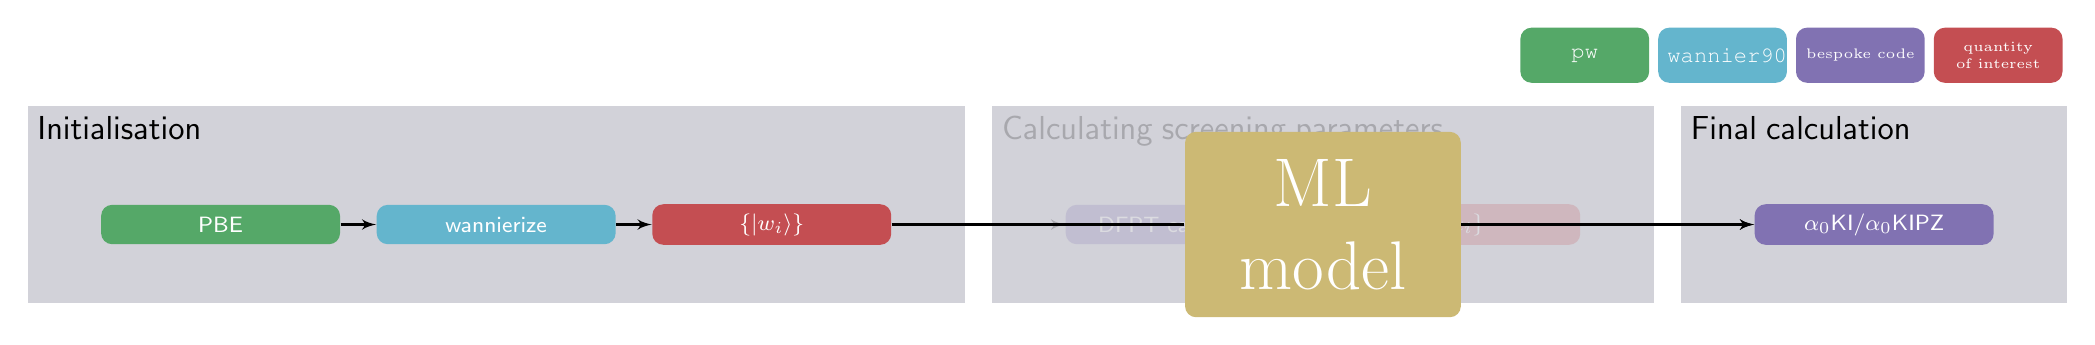
\begin{tikzpicture}[font=\tiny, x=3.5cm, y=1cm]
   \begin{pgfonlayer}{background}
      \fill [seaborn_bg_grey_dark] (-2.2,-1) rectangle (1.2,1.5);
      \node at (-2.2, 1.5) [default_text] {\large Initialisation};
      \fill [seaborn_bg_grey_dark] (1.3,-1) rectangle (3.7,1.5);
      \node at (1.3, 1.5) [default_text] {\large Calculating screening parameters};
      \fill [seaborn_bg_grey_dark] (3.8,-1) rectangle (5.2,1.5);
      \node at (3.8, 1.5) [default_text, text width=3.5cm] {\large Final calculation};
      % \fill [seaborn_bg_grey_dark] (8.1,-1) rectangle (9.1,1.5);
      % \node at (8.1, 1.5) [default_text, text width=3.5cm] {\large Postprocessing};
   \end{pgfonlayer}

   % Key
   \node at (3.45, 2.15) [pw, text width=1.4cm, minimum height=0.7cm] {\texttt{pw}};
   \node at (3.95, 2.15) [wannier90, text width=1.4cm, minimum height=0.7cm] {\texttt{wannier90}};
   \node at (4.45, 2.15) [bespoke, text width=1.4cm, minimum height=0.7cm, font=\tiny] {bespoke code};
   \node at (4.95, 2.15) [observable, text width=1.4cm, minimum height=0.7cm, font=\tiny] {quantity of interest};

   % Initialisation
   % Solids
   \node at (-1.5, 0) [pw] (pw PBE init) {PBE};
   \node at (-0.5, 0) [wannier90] (wannierize) {wannierize};
   \node at (0.5, 0) [observable] (unfold) {$\{\ket{w_i}\}$};
   \path [line] (pw PBE init) -- (wannierize);
   \path [line] (wannierize) -- (unfold);

   % Calculating screening parameters
   \node at (2, 0) [bespoke] (KC screen) {DFPT calculation};
   \node at (3, 0) [observable] (alphas) {$\{\alpha_i\}$};
   \path [line] (unfold) -- (KC screen);
   \path [line] (KC screen) -- (alphas);

   % Final calc
   \node at (4.5, 0) [bespoke] (KC ham) {$\alpha_0$KI/$\alpha_0$KIPZ};
   \path [line] (alphas) -- (KC ham);

   % \onslide<4->{
   %    \node at (1, 0) [default_text, fill=white, opacity=0.9, text opacity=1, anchor=center, minimum height=5cm, text width=7cm, execute at begin node=\setlength{\baselineskip}{30pt}] (nc text) {
   %       \huge Nicola Colonna
   %       \textbf{A20.00002} /
   %       paper in preparation
   %    };
   %    \node[right = -0.2cm of nc text, anchor=west]{\includegraphics[height=5cm]{figures/nicola_colonna.png}};
   % }
    \onslide<4->{
      \fill [seaborn_bg_grey_dark,opacity=0.8] (1.3,-1) rectangle (3.7,1.5);
      \node at (2.5, 0) [cp, fill=seaborn_yellow, font=\Huge, inner sep=10pt] (ml) {ML model};
      \path [headless_line] (unfold) -- (ml);
      \path [line] (ml) -- (KC ham);
    }
\end{tikzpicture}
}
   }

   \onslide<4->{(c) via machine learning (see Yannick Schubert's talk)} \blfootcite{DeGennaro2022,Colonna2022,Schubert2022}
   % \onslide<6>{
   %    \vspace{-0.375\paperheight}
   %    \begin{flushright}
   %       \begin{tcolorbox}[enhanced jigsaw, width=4cm, opacityback=0, colframe=seaborn_red, coltext=seaborn_red, left=3pt, bottom=3pt, top=3pt, right=3pt, tikz={rotate=30,transform shape}, boxrule=1.5mm]
   %          \begin{center}
   %             \includegraphics[height=1cm]{./figures/qe_logo_high_res_cropped.jpg}
   %             \bf \huge\ \raisebox{0.3cm}{+}\,
   %             \includegraphics[height=1cm]{./figures/python_logo.png}

   %             \bf \large OUT NOW!
   %          \end{center}
   %       \end{tcolorbox}
   %    \end{flushright}
   % }

\end{frame}

\begin{frame}{Resonance with other efforts}
   \begin{itemize}
      \item Wannier transition-state method of Anisimov and Kozhevnikov \cite{Anisimov2005}
      \item Optimally tuned hybrid functionals of Kronik, Pasquarello, and others (refer back to Leeor's talk on Wednesday) \cite{Kronik2012,Wing2021}
      \item Ensemble DFT of Kronik and co-workers \cite{Kraisler2013}
      \item Koopmans-Wannier of Wang and co-workers \cite{Ma2016}
      \item Dielectric-dependent hybrid functionals of Galli and co-workers \cite{Skone2016a}
      \item LOSC functionals of Yang and co-workers \cite{Li2018}
   \end{itemize}
\end{frame}


\begin{frame}{Koopmans compared to DFT+\emph{U}}
   \small
   \renewcommand{\arraystretch}{1.5}
   \rowcolors{1}{seaborn_bg_grey}{seaborn_bg_grey_half}
   \begin{tabularx}{\columnwidth}{L L L}
                                   & \textbf{DFT+\emph{U}}                                                       & \textbf{Koopmans}                                                                                                           \\
      \hline
      % designed to correct SIE, as defined by... & erroneous global curvature in total energies                                & dependence of $\varepsilon_i$ on $f_i \ \forall i$ \leavevmode\onslide<4->{\textcolor{red}{(canonical orbitals)}}                                                   \\
      the functional...            & corrects local curvature in total energies                                  & \leavevmode\onslide<2->{removes dependence of $\varepsilon_i$ on $f_i$ and guarantees $\varepsilon_i = E_i(N\pm 1) - E(N)$} \\
      correction applied to...     & selected subspaces only (e.g. \emph{3d} orbitals)                           & \leavevmode\onslide<3->{every variational orbital in the entire system}                                                     \\
      orbitals defined by...       & Hubbard projectors (atom-centred, frozen, incomplete)                       & \leavevmode\onslide<4->{variational (minimising) orbitals}                                                                  \\
      corrective parameters are... & $\{U^I\}$, defined with respect to charge-neutral excitations (if using LR) & \leavevmode\onslide<5->{$\{\alpha_i\}$, defined with respect to charged excitations}                                        \\
   \end{tabularx}
\end{frame}

\begin{frame}{Koopmans functionals: results for molecules}
   \small
   Ionisation potentials $ = E(N-1) - E(N) \stackrel{?}{=} -\varepsilon_{HO}$ of 100 molecules (the GW100 set) cf. CCSD(T)
   \begin{center}
      \includegraphics[height=0.2\textwidth]{figures/colonna_2019_gw100_ip}
      % \onslide<2->{\includegraphics[height=0.23\textwidth]{figures/colonna_2019_gw100_deeper}}
   \end{center}

   \vspace{-3ex}
   Ultraviolet photoemission spectra
   \begin{center}
      \begin{tikzpicture}
         \node [inner sep=0pt](fig) at (0,0) {\includegraphics[height=0.35\textheight]{figures/fig_nguyen_prl_spectra.png}};
         \draw [very thick, color=seaborn_red] (-5.35,-0.07) rectangle (5.4,1.6);
      \end{tikzpicture}
   \end{center}
   \vspace{-2ex}

   \blfootcite{Colonna2018,Nguyen2015}
\end{frame}

% \begin{frame}{Koopmans functionals: results for molecules}
%    Electron affinities $ = E(N) - E(N+1) \stackrel{?}{=} -\varepsilon_{LU}$ of molecules cf. CCSD(T)/exp
%    \vspace{2ex}
% 
%    \small
%    \begin{center}
%       For 15 of the GW100 molecules with bound LUMOs
% 
%       \includegraphics[height=0.5\textheight]{figures/fig_gw100_ea_mae_mse.pdf}
% 
%       \textcolor{seaborn_bg_grey_darker}{\footnotesize Linscott et al. (in prep)}
%    \end{center}
% \end{frame}

\begin{frame}{Koopmans functionals: results for solids}
   \begin{minipage}[c]{0.35\textwidth}
      \includegraphics[width=\textwidth]{figures/fig_nguyen_prx_bandgaps.png}
   \end{minipage}
   \hspace{1em}
   \begin{minipage}[c]{0.6\textwidth}

      \footnotesize
      Mean absolute error (eV) across prototypical semiconductors and insulators

      \vspace{1ex}
      \begin{tabular}{c S[table-format = 2.2] S[table-format = 2.2] >{\color{seaborn_red}\bfseries}S[table-format = 2.2] >{\color{seaborn_red}\bfseries}S[table-format = 2.2] S[table-format = 2.2]}
                          & {PBE} & {G\textsubscript{0}W\textsubscript{0}} & {KI} & {KIPZ} & {QSG$\tilde{\mathsf{W}}$} \\
         \midrule
         \midrule
         $E_\mathsf{gap}$ & 2.54  & 0.56                                   & 0.27 & 0.22   & 0.18                      \\
         %                                  & {MAPE (\%)} & 48.28 & 12.10      & 7.0           \\
         \midrule
         IP               & 1.09  & 0.39                                   & 0.19 & 0.21   & 0.49                      \\
         %                                  & {MAPE (\%)} & 15.58 & 5.71                                   & 2.99 & 3.14   & 7.41
      \end{tabular}
   \end{minipage}

   \blfootcite{Nguyen2018}
\end{frame}

\begin{frame}{Koopmans functionals: results for solids}
   \vspace{-0.5em}
   \begin{figure}[t]
      \centering
      \begin{subfigure}{0.45\textwidth}
         \includegraphics[width=\columnwidth]{figures/Si_kipz_bands.png}
         \caption{Si, KIPZ}
      \end{subfigure}
      \begin{subfigure}{0.45\textwidth}
         \includegraphics[width=\columnwidth]{figures/GaAs_ki_bands.png}
         \caption{GaAs, KI}
      \end{subfigure}
      % \begin{subfigure}{\textwidth}
      %    \begin{tabularx}{\columnwidth}{C C C C C C C}
      %       ZnO                                  & LDA  & HSE  & GW$_0$ & scG$\tilde{\rm W}$ & KI   & exp.      \\
      %       \hline
      %       $E_\mathsf{gap}$ (eV)                & 0.79 & 2.79 & 3.0    & 3.2                & 3.62 & 3.60      \\
      %       $\langle \varepsilon_d \rangle$ (eV) & -5.1 & -6.1 & -6.4   & -6.7               & -6.9 & -7.5/-8.0 \\
      %    \end{tabularx}
      % \end{subfigure}
   \end{figure}
   \begin{center}
      \footnotesize
      \begin{tabular}{l l S[table-format = 2.2] S[table-format = 2.2] >{\color{seaborn_red}\bfseries}S[table-format = 2.2] >{\color{seaborn_red}\bfseries}S[table-format = 2.2] >{\color{seaborn_red}\bfseries}S[table-format = 2.2] S[table-format = 2.2]}
                               &                                  & {PBE} & {QSG$\tilde{\mathsf{W}}$} & {KI} & {pKIPZ} & {\bf KIPZ} & {exp} \\
         \midrule
         \midrule
         {Si}                  & $E_\mathsf{gap}$                 & 0.55  & 1.24                      & 1.18 & 1.17    & 1.19       & 1.17  \\
         \midrule
         \multirow{2}{*}{GaAs} & $E_\mathsf{gap}$                 & 0.50  & 1.61                      & 1.53 & 1.49    & 1.50       & 1.52  \\
                               & $\langle \varepsilon_d \rangle $ & 14.9  & 17.6                      & 16.9 &         & 17.7       & 18.9
      \end{tabular}
   \end{center}
   \blfootcite{DeGennaro2022}
\end{frame}

\begin{frame}{Koopmans functionals: results for solids}
   \begin{figure}[t]
      \centering
      \begin{subfigure}{0.3\textwidth}
         \includegraphics[width=\columnwidth]{figures/ZnO_lda.png}
      \end{subfigure}
      \begin{subfigure}{0.3\textwidth}
         \includegraphics[width=\columnwidth]{figures/ZnO_hse.png}
      \end{subfigure}
      \begin{subfigure}{0.3\textwidth}
         \includegraphics[width=\columnwidth]{figures/ZnO_ki.png}
      \end{subfigure}
      \begin{subfigure}{\textwidth} %<-- changed width
         \centering
         %    \renewcommand\tabularxcolumn[1]{m{#1}}% <-- added
         %    \renewcommand\arraystretch{1.3}
         %    \setlength\tabcolsep{2pt}% <-- added
         \begin{tabular}{c S[table-format = 2.2] S[table-format = 2.2] S[table-format = 2.2] S[table-format = 2.2] >{\color{seaborn_red}\bfseries}S[table-format = 2.2] S[table-format = 2.2]}
            ZnO                                  & {LDA} & {HSE} & {GW$_0$} & {scG$\tilde{\rm W}$} & {KI} & {exp}       \\
            \hline
            $E_\mathsf{gap}$ (eV)                & 0.79  & 2.79  & 3.0      & 3.2                  & 3.62 & 3.60        \\
            $\langle \varepsilon_d \rangle$ (eV) & -5.1  & -6.1  & -6.4     & -6.7                 & -6.9 & {-7.5/-8.0} \\
         \end{tabular}
         %        \caption{table}
      \end{subfigure}
      % \caption{Band structure of ZnO calculated at different level of theory:
      %    LDA (left panel), HSE (middle panel) and KI (right panel). Shaded areas
      %    highlight valence (light blue) and conduction (light red) manifolds. The
      %    experimental values for the band gap and for the energy position of
      %    Zn $d$-states are represented by the dashed green line and by the dashed
      %    red line, respectively.
      %    Table: Band gap and position of Zn $d$ states with respect to the top of the valence band at different level of theory compared to experimental and GW results from Ref.~\onlinecite{shishkin_accurate_2007}.}
   \end{figure}
   \blfootcite{Colonna2022}
\end{frame}

\begin{frame}{How do I run these calculations?}

   \texttt{kcw.x} (DFPT implementation) is distributed in Quantum ESPRESSO v7.1 onwards

   \vspace{2ex}

   \texttt{kcp.x} (supercell implementation) is available publically

   \vspace{4ex}

   But complex workflows mean that...
   \begin{itemize}
      \item lots of different codes that need to handshake
      \item lots of scope for human error
      \item reproducibility becomes difficult
      \item expert knowledge required
   \end{itemize}

   Our solution...

\end{frame}

\begin{frame}{}
   \begin{center}
      \includegraphics[width=0.6\textwidth]{figures/koopmans_grey_on_transparent.png}
   \end{center}

   \vspace{-2ex}

   \begin{columns}
      \begin{column}{0.55\textwidth}
         \begin{itemize}
            \item beta version released earlier this year\footnotemark[1]
            \item implementations of Koopmans functionals
            \item automated workflows
                  \begin{itemize}
                     \item start-to-finish Koopmans calculations
                     \item Wannierisation
                     \item dielectric tensor
                     \item ...
                  \end{itemize}
            \item built on top of ASE\footnotemark[2]
            \item under the hood, calls \texttt{Quantum ESPRESSO}
            \item does not require expert knowledge
         \end{itemize}
      \end{column}

      \begin{column}{0.4\textwidth}
         \centering
         \url{koopmans-functionals.org}
         \includegraphics[width=\columnwidth]{figures/website_cropped.png}
      \end{column}
   \end{columns}
   \footnotetext[1]{Linscott et al., in prep}
   \footnotetext[2]{\cite{Larsen2017}}
\end{frame}

\begin{frame}{koopmans: the input file}
   \begin{minipage}[t]{0.475\columnwidth}
      \inputminted[fontsize=\tiny,breaklines,lastline=20]{json}{scripts/si.json}
   \end{minipage}
   \hspace{0.025\textwidth}
   \begin{minipage}[t]{0.475\columnwidth}
      \inputminted[fontsize=\tiny,breaklines,firstline=21]{json}{scripts/si.json}
   \end{minipage}
\end{frame}

% \begin{frame}{koopmans: the output file}
%    \vspace{-2ex}
%    \only<1>{
%       \inputminted[fontsize=\scriptsize,breaklines]{text}{scripts/si_ki_full.out}
%    }
%    \only<2>{
%       \inputminted[fontsize=\scriptsize,breaklines,firstline=25]{text}{scripts/si_ki_full.out}
%    }
%    \only<3>{
%       \inputminted[fontsize=\scriptsize,breaklines,firstline=50]{text}{scripts/si_ki_full.out}
%    }
%    \only<4>{
%       \inputminted[fontsize=\scriptsize,breaklines,firstline=75]{text}{scripts/si_ki_full.out}
%    }
% \end{frame}

\begin{frame}{koopmans is scriptable}
   \vspace{-2ex}
   \inputminted[fontsize=\scriptsize,breaklines]{python}{scripts/si.py}
\end{frame}

\begin{frame}{Take home messages}

   \includegraphics[height=0.2\paperheight]{figures/colonna_2019_gw100_ip.jpeg}
   \hfill
   \includegraphics[height=0.2\paperheight]{figures/fig_nguyen_prx_bandgaps.png}
   \hfill
   \adjustbox{height=0.2\paperheight}{\input{supercell_workflow.tex}\end{tikzpicture}}

   \begin{itemize}
      \item Koopmans functionals are a class of functionals that treat spectral properties on the same footing as total energy differences (via GPWL)
      \item they can give orbital energies and band structures with comparable accuracy to state-of-the-art GW
      \item Koopmans functionals are implemented in \texttt{Quantum ESPRESSO}, and we can use \texttt{koopmans} to run these calculations easily
   \end{itemize}

\end{frame}

\begin{frame}{Acknowledgements}

   \begin{center}
      \footnotesize
      \begin{tabularx}{0.7\textwidth}{CCCC}
         \includegraphics[height = 0.2\paperheight]{figures/nicola_marzari.jpg}     &
         \includegraphics[height = 0.2\paperheight]{figures/nicola_colonna2.png}    &
         \includegraphics[height = 0.2\paperheight]{figures/riccardo_degennaro.jpg} &
         \includegraphics[height = 0.2\paperheight]{figures/yannick_schubert.jpg}     \\
         % \includegraphics[height = 0.2\paperheight]{figures/daniel_cole.jpeg}       &
         % \includegraphics[height = 0.2\paperheight]{figures/mike_payne.jpeg}        &
         % \includegraphics[height = 0.2\paperheight]{figures/david_oregan.jpg}         \\
         Nicola Marzari                                                             &
         Nicola Colonna                                                             &
         Riccardo De~Gennaro                                                        &
         Yannick Schubert                                                             \\
      \end{tabularx}
   \end{center}
   \begin{center}
      \includegraphics[height = 0.125\paperheight]{logos/SNF_logo_standard_print_color_pos_e.eps}
      \hspace{1em}
      \includegraphics[height = 0.125\paperheight]{figures/marvel_trimmed.png}
   \end{center}

   \vspace{1ex}
   \begin{center}
      Follow \includegraphics[height=\fontcharht\font`\B]{figures/Twitter_Bird.png} \textcolor{twitter_blue}{@ed\_linscott} for updates | Slides available at \includegraphics[height=\fontcharht\font`\B]{logos/github-favicon.png} github/elinscott
   \end{center}


   % \begin{multicols}{2}
   %    \tiny
   %    \printbibliography
   %    \normalsize
   % \end{multicols}
   \vspace{2ex}
   \scriptsize

   \setbeamercolor*{bibliography entry title}{fg=black}
   \setbeamercolor*{bibliography entry author}{fg=black}
   \setbeamercolor*{bibliography entry location}{fg=black}
   \setbeamercolor*{bibliography entry note}{fg=black}

   \vspace{2ex}
   \scriptsize
\end{frame}

\backupbegin
\begin{frame}{}

   \begin{center}
      \huge SPARE SLIDES
   \end{center}

\end{frame}

\begin{frame}{Koopmans functionals: off-diagonal occupancies}
   \begin{block}{Recap from earlier}
      Key idea: construct a functional such that the \emph{variational} orbital energies
      \begin{equation*}
         \varepsilon^\mathsf{Koopmans}_i = \braopket{\varphi_i}{H}{\varphi_i} = \partial E_\mathsf{Koopmans}/\partial f_i
      \end{equation*}
      are...
      \begin{itemize}
         \item independent of the corresponding occupancies $f_i$
         \item equal to the corresponding total energy difference $E_i(N-1) - E(N)$
      \end{itemize}
   \end{block}

   zero band gap $\rightarrow$ occupancy matrix for variational orbitals is off-diagonal
\end{frame}


% \begin{frame}{References}
%    \setbeamercolor*{bibliography entry title}{fg=black}
%    \setbeamercolor*{bibliography entry author}{fg=black}
%    \setbeamercolor*{bibliography entry location}{fg=black}
%    \setbeamercolor*{bibliography entry note}{fg=black}
%    \printbibliography
%    % For further reading on Koopmans functionals, see \cite{Dabo2010,Borghi2014,Nguyen2018,Colonna2018,Colonna2019,DeGennaro2022,Colonna2022}
% 
% \end{frame}
% \begin{frame}{Learning the screening parameters}
%    \begin{center}
%       \begin{tikzpicture}
%          \node[inner sep=0pt] (water box) at (0,0)
%          {
%             \includegraphics[width=0.25\textwidth]{figures/orbital.emp.00191_cropped.png}
%          };
%          \node[below=0cm of water box] (density) {$\rho_i(\mathbf{r})$};
%          \node[right=0.2\textwidth of water box] (power spectrum) {
%             $
%                \begin{bmatrix}
%                   x_{0} \\
%                   x_{1} \\
%                   x_{2} \\
%                   \vdots
%                \end{bmatrix}
%             $
%          };
%          \path[line] (water box) -- node [midway, above, align=center] (decomposition) {power spectrum \\ decomposition} (power spectrum);
%          \node[right=0.2\textwidth of power spectrum] (screening parameter) {$\alpha_i$};
%          \path[line] (power spectrum) -- node [midway, above, align=center] (model) {ML model} (screening parameter);
%       \end{tikzpicture}
%    \end{center}
% 
%    \vspace{-4em}
% 
%    \blfootcite{Schubert2022}
% 
%    \begin{align*}
%       c^i_{nlm,k=\mathsf{orbital}} & =\int d\textbf{r} g_{nl}(r)Y_{lm}(\theta,\varphi)\rho^i(\textbf{r}-\textbf{R}^i)                        \\
%       p^i_{n_1n_2l,k_1k_2}         & =\pi \sqrt{\frac{8}{2l+1}}\sum\limits_m {c_{n_1lm,k_1}^{i *}}c_{n_2lm,k_2}^i \label{eq: power spectrum}
%    \end{align*}
% 
%    % $g_{nl}$ = orthonormalised radial Gaussian basis functions
% 
%    % $Y_{lm}$ = spherical harmonics
% 
% \end{frame}
% 
% \begin{frame}{Learning the screening parameters}
%    \begin{center}
% 
%       \includegraphics[height=0.7\paperheight]{figures/CsSnI3_calc_vs_pred_Edward.png}
%       \includegraphics[height=0.7\paperheight]{figures/convergence_analysis_Edward.png}
% 
%       loss of accuracy of the band gap of $\sim$ 0.02 eV
% 
%       (cf. when calculating screening parameters \emph{ab initio})
% 
%       speedup of 70$\times$
%    \end{center}
% 
%    \blfootcite{Schubert2022}
% 
% \end{frame}


\backupend
\end{document}
